\documentclass[a4paper, landscape]{article}

\usepackage[a4paper, margin = 0.5em, landscape]{geometry}

\usepackage{tikz}
\usetikzlibrary{angles,quotes,decorations.pathmorphing}

\tikzset{snake it1/.style = {decorate, decoration = {snake , segment length = 21.3mm , amplitude = 2mm}}}
\tikzset{snake it2/.style = {decorate, decoration = {snake , segment length = 9.8mm , amplitude = 2mm}}}
\tikzset{snake it3/.style = {decorate, decoration = {snake , segment length = 5.25mm , amplitude = 2mm}}}
\tikzset{snake it4/.style = {decorate, decoration = {snake , segment length = 2mm , amplitude = 2mm}}}

\usepackage{amsmath}
\usepackage{xcolor}

\title{}
\author{}
\date{}

\begin{document}

\pagenumbering{gobble}

\centering

\vspace*{\fill}

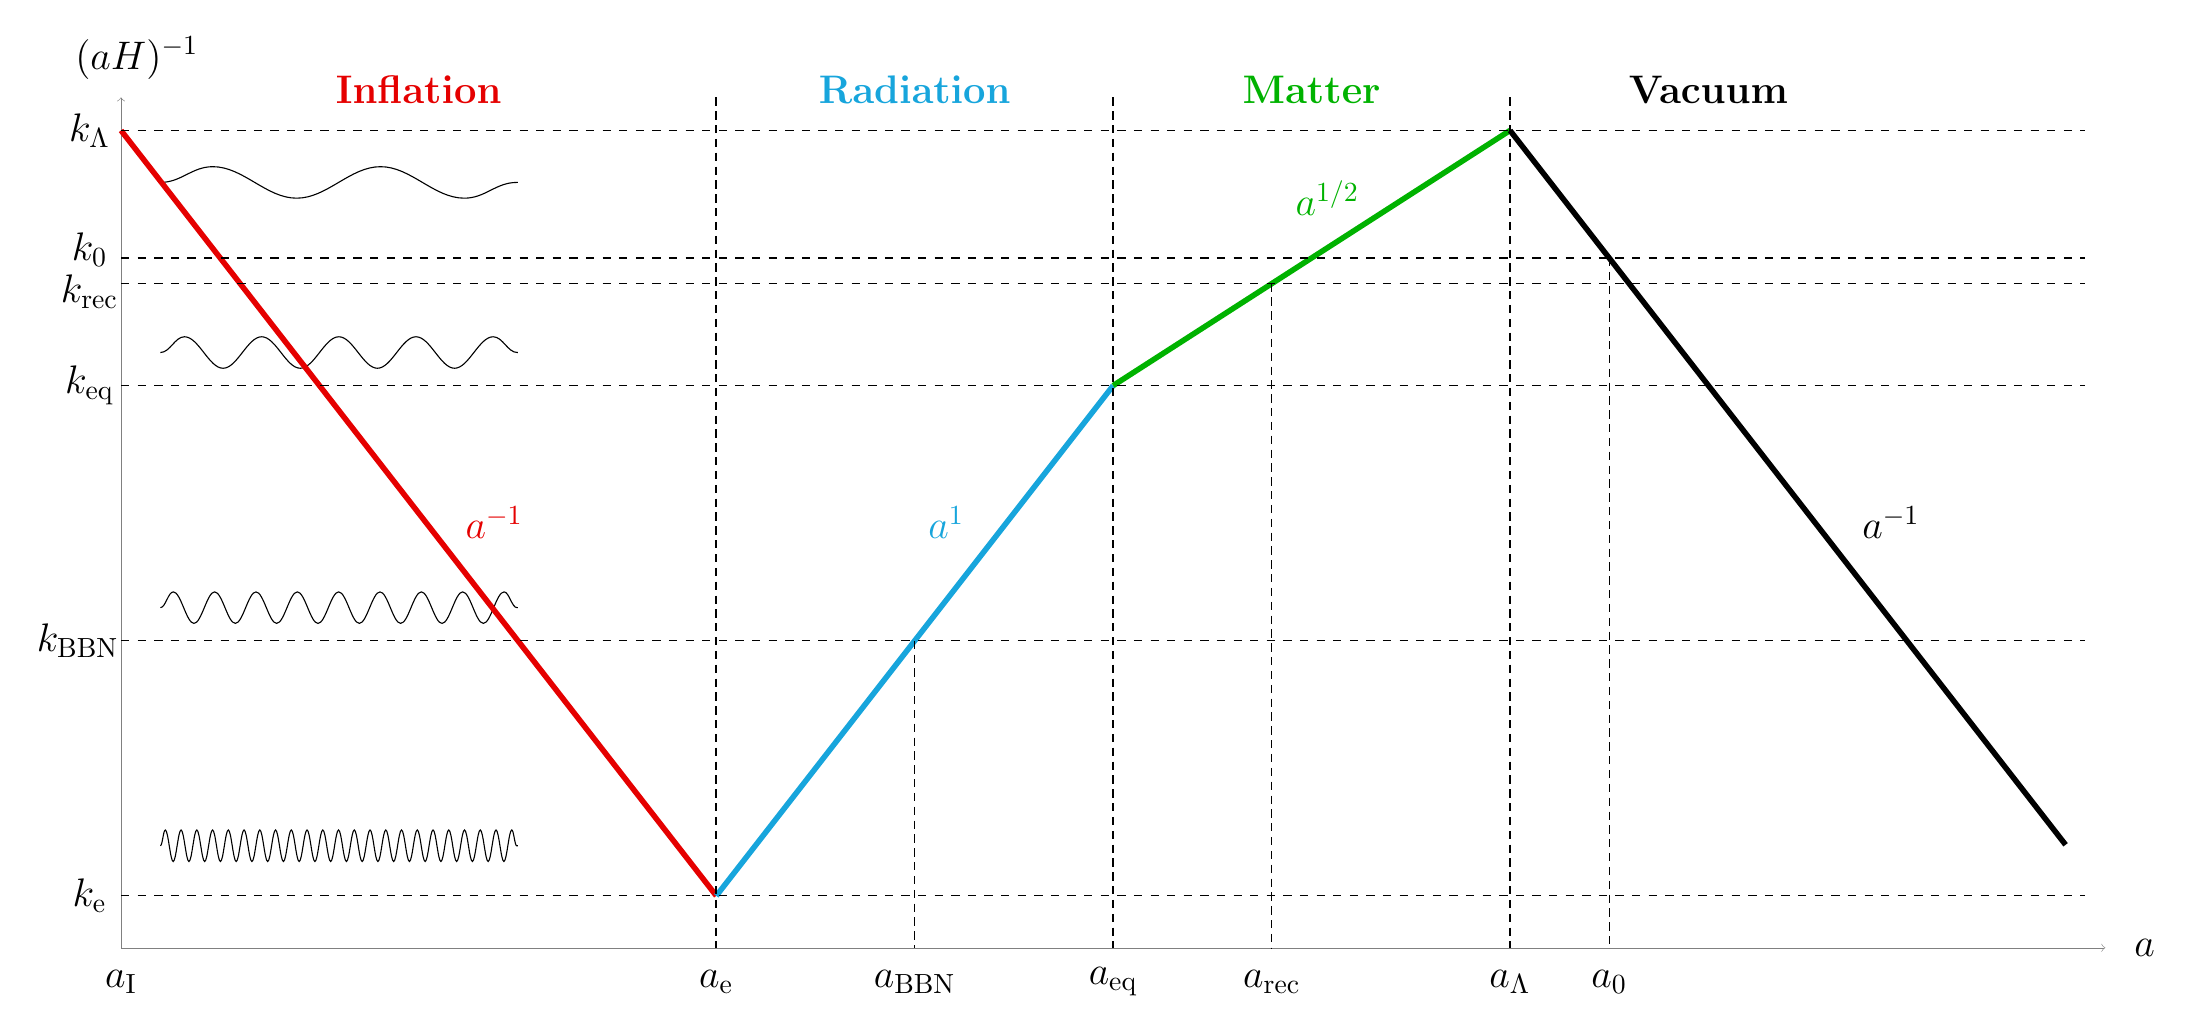
\begin{tikzpicture}

  \def\scale{18}
  \def\yscale{\scale * 0.6}
  \def\xscale{\scale * 1.4}
  \def\offset{1.5}

  \draw [help lines,->] (0 , 0) -- (\xscale , 0);
  \draw [help lines,->] (0 , 0) -- (0 , \yscale);

  \path [draw = black, snake it1] (0.5 , \yscale * 0.9) -- (\xscale * 0.2 , \yscale * 0.9);
  \path [draw = black, snake it2] (0.5 , \yscale * 0.7) -- (\xscale * 0.2 , \yscale * 0.7);
  \path [draw = black, snake it3] (0.5 , \yscale * 0.4) -- (\xscale * 0.2 , \yscale * 0.4);
  \path [draw = black, snake it4] (0.5 , \yscale * 0.12) -- (\xscale * 0.2 , \yscale * 0.12);

  \node at (\xscale + 0.5 , 0) {\Large $ a $};
  \node at (0.2 , \yscale + 0.5) {\Large $ (aH)^{-1} $};

  \draw [line width = 2pt, draw = red!90!black] (0 , \yscale * 1.1 - \offset) -- (\xscale * 0.3 , \yscale * 0.2 - \offset);
  \draw [line width = 2pt, draw = cyan!90!black] (\xscale * 0.3 , \yscale * 0.2 - \offset) -- (\xscale * 0.5 , \yscale * 0.8  - \offset);
  \draw [line width = 2pt, draw = green!70!black] (\xscale * 0.5 , \yscale * 0.8 - \offset) -- (\xscale * 0.7 , \yscale * 1.1 - \offset);
  \draw [line width = 2pt, draw = black] (\xscale * 0.7 , \yscale * 1.1 - \offset) -- (\xscale * 0.98 , \yscale * 0.26 - \offset);

  \draw [thick, densely dashed] (\xscale * 0.3 , \yscale) -- (\xscale * 0.3 , 0);
  \draw [thick, densely dashed] (\xscale * 0.5 , \yscale) -- (\xscale * 0.5 , 0);
  \draw [thick, densely dashed] (\xscale * 0.7 , \yscale) -- (\xscale * 0.7 , 0);

  \node at (0 , - \yscale * 0.04) {\Large $ a_\text{I} $};
  \node at (\xscale * 0.3 , - \yscale * 0.04) {\Large $ a_\text{e} $};
  \node at (\xscale * 0.5 , - \yscale * 0.04) {\Large $ a_\text{eq} $};
  \node at (\xscale * 0.7 , - \yscale * 0.04) {\Large $ a_\Lambda $};

  \draw [thin, densely dashed] (\xscale * 0.40 , \yscale * 0.50 - \offset) -- (\xscale * 0.40 , 0);
  \draw [thin, densely dashed] (\xscale * 0.58 , \yscale * 0.92 - \offset) -- (\xscale * 0.58 , 0);
  \draw [thin, densely dashed] (\xscale * 0.75 , \yscale * 0.95 - \offset) -- (\xscale * 0.75 , 0);

  \node at (\xscale * 0.40 , - \yscale * 0.04) {\Large $ a_\text{BBN} $};
  \node at (\xscale * 0.58 , - \yscale * 0.04) {\Large $ a_\text{rec} $};
  \node at (\xscale * 0.75 , - \yscale * 0.04) {\Large $ a_0 $};

  \draw [thin, dashed] (0 , \yscale * 0.2 - \offset) -- (\xscale * 0.99 , \yscale * 0.2 - \offset);
  \draw [thin, dashed] (0 , \yscale * 0.5 - \offset) -- (\xscale * 0.99 , \yscale * 0.5 - \offset);
  \draw [thin, dashed] (0 , \yscale * 0.8 - \offset) -- (\xscale * 0.99 , \yscale * 0.8 - \offset);
  \draw [thin, dashed] (0 , \yscale * 0.92 - \offset) -- (\xscale * 0.99 , \yscale * 0.92 - \offset);
  \draw [thin, dashed] (0 , \yscale * 0.95 - \offset) -- (\xscale * 0.99 , \yscale * 0.95 - \offset);
  \draw [thin, dashed] (0 , \yscale * 1.1 - \offset) -- (\xscale * 0.99 , \yscale * 1.1 - \offset);

  \node at (- 0.4 , \yscale * 0.2 - \offset) {\Large $ k_\text{e} $};
  \node at (- 0.55 , \yscale * 0.5 - \offset) {\Large $ k_\text{BBN} $};
  \node at (- 0.4 , \yscale * 0.8 - \offset) {\Large $ k_\text{eq} $};
  \node at (- 0.4 , \yscale * 0.91 - \offset) {\Large $ k_\text{rec} $};
  \node at (- 0.4 , \yscale * 0.96 - \offset) {\Large $ k_0 $};
  \node at (- 0.4 , \yscale * 1.1 - \offset) {\Large $ k_\Lambda $};

  \node at (\xscale * 0.15 , \yscale + 0.1) {\textcolor{red!90!black}{\Large \bfseries Inflation}};
  \node at (\xscale * 0.40 , \yscale + 0.1) {\textcolor{cyan!90!black}{\Large \bfseries Radiation}};
  \node at (\xscale * 0.60 , \yscale + 0.1) {\textcolor{green!70!black}{\Large \bfseries Matter}};
  \node at (\xscale * 0.80 , \yscale + 0.1) {\textcolor{black}{\Large \bfseries Vacuum}};

  \node at (\xscale * 0.2 - 0.3 , \yscale * 0.5) {\textcolor{red!90!black}{\Large $ a^{-1} $}};
  \node at (\xscale * 0.4 + 0.4 , \yscale * 0.5) {\textcolor{cyan!90!black}{\Large $ a^{1} $}};
  \node at (\xscale * 0.6 + 0.2 , \yscale * 0.9 - 0.2) {\textcolor{green!70!black}{\Large $ a^{1/2} $}};
  \node at (\xscale * 0.9 - 0.2 , \yscale * 0.5) {\textcolor{black}{\Large $ a^{-1} $}};

\end{tikzpicture}

\vspace*{\fill}

\end{document}
